\documentclass[a4paper,10pt]{article}

\usepackage[utf8]{inputenc}
\usepackage[T1]{fontenc}
\usepackage[absolute]{textpos}
\usepackage{changepage}
\usepackage{ulem}
\usepackage{blindtext}
\usepackage{rotating}
\usepackage{hanging}
\usepackage{nopageno}
\usepackage{circledsteps}
\usepackage{latexsym}
\usepackage{parskip}
\usepackage{soul}
\usepackage{stackengine}
\usepackage{stix}
\usepackage{tikz}
\usepackage{transparent}
\usepackage{xcolor}
\usepackage[paperwidth=5.5in, paperheight=16in, top=0.7in, left=0.7in, right=0.7in, bottom=0.1in]{geometry}
\usetikzlibrary{arrows.meta,decorations.pathreplacing,calligraphy}

\newcommand{\ulfelttip}[1]{%
    \tikz[baseline=(to_underline.base)]{
        \color{red}
        \node[inner sep=0pt,outer sep=0pt] (to_underline) {#1};
        \draw[line width=0.05in, opacity=0.6] ([xshift=1pt,yshift=-2pt]to_underline.south west) -- ([xshift=-1pt,yshift=-2pt]to_underline.south east);
    }%
}%
\newcommand{\multilinerightbrace}{
	\begin{tikzpicture}[remember picture,overlay]
		\draw [pen colour ={blue},
		decorate, 
		decoration = {calligraphic brace}
		] (0.7,0.3) -- (0.7,-0.5);
	\end{tikzpicture}
}

\newcommand{\twoabove}{
    
\begin{tikzpicture}[remember picture,overlay]
        \node[] at (0.3,0.3) {2};
    \end{tikzpicture}
}

\newcommand{\threeabove}{
    
\begin{tikzpicture}[remember picture,overlay]
        \node[] at (0.2,0.25) {3};
    \end{tikzpicture}
}

\newcommand{\downarrowabove}{
    
\begin{tikzpicture}[remember picture,overlay]
        \node[] at (0.275,0.25) {$\downarrow$};
    \end{tikzpicture}
}

\newcommand{\leftarrowabove}{
    \begin{tikzpicture}[remember picture,overlay]
        \node[] at (0.8,0.3) {$\leftarrow$};
    \end{tikzpicture}
}

\newcommand{\howgreatarrow} {
    \begin{tikzpicture}[remember picture,overlay]
        \color{black}
        \draw[<->] (-5, 0.6) .. controls (-4, 0.5) and (-0.5, 0.5) .. (0.15, 0.1);
    \end{tikzpicture}\
}

\newcommand{\geraniumline} {
    \begin{tikzpicture}[remember picture,overlay]
        \draw (0.5,-0.1) -- (-0.5, -0.9);
    \end{tikzpicture}
}

\newcommand{\taylormaculatumline}{
    
\begin{tikzpicture}[remember picture,overlay]
        \draw (-0.1,0) .. controls (-0.5, -0.8) .. (-0.1, -1.5);
    \end{tikzpicture}
}

\newcommand{\catnipgenerallyarrow}{
    \begin{tikzpicture}[remember picture,overlay]
        \color{red}
        \draw[<->] (1, 0.2) .. controls (4.2, 0.3) and (4.2, -2).. (3.5, -2.5);
    \end{tikzpicture}
}

\newcommand{\shortvowelstress}{
    \begin{tikzpicture}[remember picture,overlay]
        \color{blue}
        \node[] at (0.1,0.15) {{\u{}}};
        \color{red}
        \node[] at (0.1,0.25) {{\'{}}};
    \end{tikzpicture}
}

\newcommand{\shortvowel}{
    \begin{tikzpicture}[remember picture,overlay]
        \color{blue}
        \node[] at (0.1,0.15) {{\u{}}};
    \end{tikzpicture}
}

%dimensions 5in by 7.75; I have altered to bring in line with p.20 layout]
\renewcommand{\labelitemi}{-}
\setulcolor{red}

\begin{document}
\color{blue}
\begin{flushright}
\Circled{Notes \& orig. drafts \{\sout{x}\} page 1}\par
\end{flushright}
\begin{flushleft}
\color{red} 
\begin{turn}{25}%
* See \ul{Taylor p215} 
\end{turn}
\ul{80 Flowers} (possible substitutes\par
\color{red}
for the 80 listed on pp I-VI)\par 
\color{red}
\small
% line (join "See" and 3)

\begin{tikzpicture}[remember picture,overlay]
    \color{red}
    \draw (0, 0) .. controls (-1, 1) .. (0, 2);
\end{tikzpicture}
\Circled{3} perennial .. weedy .. Eurasian .. poppy family .. {$\stackrel{\hbox{called also}}{\hbox{killwort sightwort}}$}\par
%above lines not great at the moment in making clear where LZ starts new line for space, squeezes in a bit on the right etc
\Circled{2} the lesser celandine or pilewort, still used in home med. for piles\par
``occurs locally in Eastern states.\par
\begin{itemize}
\color{blue}
\setulcolor{blue}
\normalsize
\item Celandine, \ul{Chelidonium majus} (\ul{Kamm}\par
\footnotesize 
\color{red}
swallowort - Lewis \& Short\par
\color{blue}
\normalsize
\color{red}
\Circled{$\stackrel{\hbox{{*See:}}}{\hbox{\color{blue}{pp.40-42}}}$} \color{blue}Port Jefferson planted Oct 18/74)\par
\color{red}
\small
\Circled{1} (Wordsworth's
\begin{tikzpicture}[remember picture,overlay]
    \color{red}
    \draw[->] plot [smooth] coordinates {(-1.5, -0.1) (-4, 0) (-4, 2) (-2.8, 3)};
\end{tikzpicture}
\setulcolor{red}
 poems refer to \ul{Ranunculus ficaria}, a crowfoot.$\multilinerightbrace$\par
\setulcolor{blue}
% tick
\begin{tikzpicture}[remember picture,overlay]
    \color{red}
    \draw (1.2, 1) --  (2, -0.5) -- (4.4, 7);
\end{tikzpicture}
see \# 65 v.i. pV 
%entry for 65 is on pV of working notebook, but gives sage
\color{blue}
\hfill
$\uparrow$ L = little frog $\stackrel{\hbox{Buttercup}}{\hbox{(i.e. meadow habit)}}$
%arrow should point to Ranunculus
\rule{10cm}{0.01cm}
\normalsize
\item Lavender cotton, \ul{Santolina chamaecypar-} \par
\ul{-issus} \ul{Kamm} p 206 illust \#25 Pt. J, planted\par 
%looks v like a new entry for -issus but clearly cont from previous line

\color{blue}
\normalsize
Oct 18/74
\small
\color{red}
\tiny
$\downarrowabove$
\small
John 
\tiny
$\leftarrowabove$
\small
\setulcolor{red}
Parkinson 1629 \ul{Paradisus Terrestis}\par 
\setulcolor{blue}
``The rarity \& novelty of this herb, being\par
for the most part but in the gardens of great persons, doth\par
cause it to be of great regard''
%LZ tweaking the quotation?
\color{blue}
\normalsize
\item Spearmint
\vspace{0.2cm}

\begin{tikzpicture}[remember picture,overlay]
    \color{red}
    \draw (-0.8,0.3) --  (-0.5, -0.1) -- (0.5, 0.5);
\end{tikzpicture}
(Pt. J. 

\begin{tikzpicture}[remember picture,overlay]
    \color{red}
    \draw (-0.8,0.3) --  (-0.5, -0.1) -- (0.5, 0.5);
\end{tikzpicture}
planted 

\begin{tikzpicture}[remember picture,overlay]
    \color{red}
    \draw (-0.8,0.3) --  (-0.5, -0.1) -- (0.5, 0.5);
\end{tikzpicture}
ea. Oct 74)

\begin{tikzpicture}[remember picture,overlay]
    \color{red}
    \draw (-0.8,0.3) --  (-0.5, -0.1) -- (0.5, 0.5);
\end{tikzpicture}
\item Sp\ul{ider}

\begin{tikzpicture}[remember picture,overlay]
    \color{red}
    \draw (-0.8,0.3) --  (-0.5, -0.1) -- (0.5, 0.5);
\end{tikzpicture}
pl\ul{ant} 

\begin{tikzpicture}[remember picture,overlay]
    \color{red}
    \draw (-0.8,0.3) --  (-0.5, -0.1) -- (0.5, 0.5);
\end{tikzpicture}
(lily family)
\item \ulfelttip{\color{blue} thyme} (\ulfelttip{\color{blue}\ul{time}}) (Pt. J. {$\stackrel{\hbox{Aug-}}{\hbox{Sep}}$}74) ($\stackrel{\hbox{see \#70}}{\hbox{pVI v.i}}$
\begin{tikzpicture}[remember picture,overlay,line width=0.05in,opacity=0.6]
    \color{red}
    \draw (-6.7,0) --  (-6.5, -0.1) -- (-6, 0.5);
\end{tikzpicture}
\begin{tikzpicture}[remember picture,overlay,line width=0.05in,opacity=0.6]
    \color{red}
    \draw (-4.3,0) --  (-4.1, -0.1) -- (-3.6, 0.5);
\end{tikzpicture}
\begin{tikzpicture}[remember picture,overlay,line width=0.05in,opacity=0.6]
    \color{red}
    \draw (-1.1,0) --  (-0.9, -0.1) -- (-0.4, 0.5);
\end{tikzpicture}
\item (\ul{mint} 

\begin{tikzpicture}[remember picture,overlay]
    \color{blue}
    \draw (-0.8,0.3) --  (-0.1, -0.6);
    \draw (-0.1, 0.3) -- (-0.8,-0.6);
\end{tikzpicture}
\ul{geranium} 

\begin{tikzpicture}[remember picture,overlay]
    \color{blue}
    \draw (-0.8,0.3) --  (-0.1, -0.6);
    \draw (-0.1, 0.3) -- (-0.8,-0.6);
\end{tikzpicture}
or costmary 

\begin{tikzpicture}[remember picture,overlay]
    \color{blue}
    \draw (-0.8,0.3) --  (-0.1, -0.6);
    \draw (-0.1, 0.3) -- (-0.8,-0.6);
\end{tikzpicture}Pt. J 

\begin{tikzpicture}[remember picture,overlay]
    \color{blue}
    \draw (-0.8,0.3) --  (-0.1, -0.6);
    \draw (-0.1, 0.3) -- (-0.8,-0.6);
\end{tikzpicture}
Oct 

\begin{tikzpicture}[remember picture,overlay]
    \color{blue}
    \draw (-0.8,0.3) --  (-0.1, -0.6);
    \draw (-0.1, 0.3) -- (-0.8,-0.6);
\end{tikzpicture}
26/74

\begin{tikzpicture}[remember picture,overlay]
    \color{blue}
    \draw (-0.8,0.3) --  (-0.1, -0.6);
    \draw (-0.1, 0.3) -- (-0.8,-0.6);
\end{tikzpicture}\par 
Chrysanthemum Balsamita Garden Ency Taylor)
\begin{tikzpicture}[remember picture,overlay]
    \color{blue}
    \draw (-6, 0.3) --  (-5.5, -0.5) -- (0, 14);
\end{tikzpicture}
\begin{adjustwidth}{-0.5in}{-0.5in}
    \rule{4.5in}{0.005in}  
\end{adjustwidth}
\begin{tikzpicture}[remember picture,overlay,line width=0.05in,opacity=0.6]
    \color{red}
    %tick-cross
    \draw (-1.1,1.7) --  (-0.4, 1);
    \draw (-0.4,1.7) -- (-1.1,1) -- (-1.3,1.3);
    %smaller cross
    \draw (-1.7,1.8) --  (-1.3, 1.4);
    \draw (-1.3,1.8) -- (-1.7,1.4);
\end{tikzpicture}
\begin{tikzpicture}[remember picture,overlay]
    \color{blue}
    \draw[->] (0.9, 0.7) -- (0.9, -0.2);
\end{tikzpicture}
%this item crossed out; probably Balsamita, but doesn't quite look like it; line down to
\hspace{0.5in}(identified as follow at {$\stackrel{\hbox{Suffolk}}{\hbox{Rose Soc.}}$})
\item sweet-fern (Comptonia, \ul{Taylor}; resembles\par 
spleenwort (a fern) but \ul{sweet-fern} is\par 
a shrub of the walnut family - see Gray)\par
Oct 28/74 Pt..J.\par
\color{red}
\footnotesize
\begin{minipage}{2in} 
    $\taylormaculatumline$Taylor lists wild $\geraniumline$geranium under\par
    \setulcolor{red}
    \ul{geraniaceae} - a {\Longunderstack{separate family}}\par
    \setulcolor{blue}
\end{minipage}%
\hfill
\begin{minipage}{0.6in}
    Gray $\stackrel{\hbox{817-}}{\hbox{p818}}$ 
\end{minipage}%
\begin{minipage}{0.7in}
    under\par
    g\'eum\par
    (Rose family)
\end{minipage}%
\begin{tikzpicture}[remember picture,overlay]
    \color{red}
    \draw[->] (-1.8,-0.3) -- (-4, -1);
\end{tikzpicture}
%Gray has Geum with grave, but LZ's looks acute
\color{blue}
\normalsize
\item wild geranium (\ul{Taylor}, \ul{Ge}\setulcolor{red}r\ul{anium} \ul{macu}la-\par
\ul{tum}; also called alumsroot
\color{red}
* 
\color{blue}
\& chocolateflower\par
\color{blue}
\setstcolor{red}
[\st{no relation to those}]
\begin{tikzpicture}[remember picture,overlay]
    \color{red}
    \draw[->] (-0.1, 0.1) .. controls (-1.5, 0) .. (-3, 0.25);
\end{tikzpicture}
(Pt. J {$\stackrel{\hbox{identified*}}{\hbox{Oct 30/74}}$}\par
[*neighbor called it wild strawberry, but\par 
no berry]\par
%should have square brackets from [*neighbor to berry] but was confusing LaTeX
Gray - The name of a nymph etc orig a water plant\par 
sour gum, pepperidge \color{red} (\ul{Cheyney}, What Tree is That?)
\color{blue}
\item Nyssa sylvatica Pt J 306 {$\stackrel{\hbox{- identified?}}{\hbox{E Brway Nov 3/74}}$}
\begin{tikzpicture}[remember picture,overlay]
    \draw[red] (-6.5,-0.3) rectangle (3,1.8);
\end{tikzpicture}
\begin{adjustwidth}{-0.5in}{-0.5in}
    \rule{4.5in}{0.005in}  
\end{adjustwidth}


\item Catnip - Same as \underline{Glecoma} hederacea (Taylor)\par
\setulcolor{red}
\& \#29 pg III v.i. ``The $\catnipgenerallyarrow$\ulfelttip{\color{red}\Circled{\color{blue}catnip} \color{blue} and the} \par
\ulfelttip{\color{blue}amaranth! - man's} \ulfelttip{\color{blue}earthly household} \par
\ulfelttip{\color{blue}peace} \& \ulfelttip{\color{blue}the ever-encroaching appetite} \ulfelttip{\color{blue}for God}''\par
\setulcolor{blue}
Melville, \ul{Pierre} Bk xxv IV (p386 \ul{Signet} ed.)
\color{red}
\begin{adjustwidth}{-0.5in}{-0.5in}
catnip L N$\shortvowelstress$ep$\shortvowel$eta %more accents 
Catmint .. per. \& ann. herbs .. \sout{tall}\par
\sout{tall erect or trailing} tall \& erect, or dwarf trailing, generally (over)
\end{adjustwidth}
\end{itemize}
\end{flushleft}
\begin{tikzpicture}[remember picture,overlay,line width=0.05in,opacity=0.6]
    \color{red}
    \draw (0.3, 4.5) -- (0.3, 1.7);
    \draw (-0.3,2.4) --  (0, 1.7) -- (1.5, 4.5);
    \draw (0.8,1.7) --  (1.5, 0.7) -- (3.5, 4.5);
    \draw (2.3,1.7) --  (3, 0.7) -- (5, 4.5);
    \draw (4.8,1.7) --  (5.5, 0.7) -- (7.5, 4.5);
\end{tikzpicture}

%absolute positioned text
% orig. note (top right)
\begin{textblock*}{5cm}(11cm,2.5cm)%
	\begin{minipage}{5cm} 
        \color{blue} 
        \Circled{{$\stackrel{\hbox{orig p \#}}{\hbox{I A-B}}$}}\par		
	\end{minipage}%
\end{textblock*}%

\begin{textblock*}{5cm}(0.2cm,10.5cm)%
    \footnotesize
    \color{red}
            \rotatebox{15}{
            \fcolorbox{black}{white}{
                \begin{minipage}{1.5cm}
                \vspace{0.2cm}
                How {\Longstack{\tiny$\twoabove$\footnotesize
                great fallen}}\par 
                \tiny$\threeabove$\footnotesize
                are the great\par 
                L.Z.
                \end{minipage}
            }
        }
\end{textblock*}%
\begin{textblock*}{5cm}(6.5cm,12.8cm)%
    \color{black}
    $\howgreatarrow$
    \footnotesize{i.e. LZ How great are the fallen}
\end{textblock*}%

\begin{textblock*}{5cm}(1.5cm,14cm)%
	\begin{minipage}{5cm} 
        \small
        \color{red}
        See \#68
	\end{minipage}%
\end{textblock*}%

\begin{textblock*}{5cm}(5cm,13.8cm)%
	\begin{minipage}{5cm} 
        \footnotesize
        \color{red}
        \setstackgap{S}{0.5pt}
        Gk = {\Shortstack{green plant}} chlorophytum\par
        \vspace{0.2cm}
        exalted - elated elatum
	\end{minipage}%
\end{textblock*}%

\begin{textblock*}{5cm}(1.5cm,16.1cm)%
    \begin{minipage}{5cm} 
        \large
        \color{red}
        \transparent{0.6}
        \textbf{?}
        \transparent{1}
        \color{blue}
        ??
    \end{minipage}%
\end{textblock*}%

\setulcolor{blue}
\color{red}
\begin{textblock*}{5cm}(0.5cm,21.2cm)%
    \small
    \begin{minipage}{5cm} 
        \color{red}
        \setulcolor{red}
        but $\stackrel{\hbox{is}}{\hbox{$\caretinsert$}}$ not $\ast$\par
        \ul{Heuchera}\par
        also called\par
         alumroot\par
        (saxifrage\par
        family)
        \normalsize
    \end{minipage}%
\end{textblock*}%

\begin{textblock*}{2in}(0.9cm,24.8cm)%
    \small
    \begin{minipage}{2in} 
        \color{blue}
        See\par
        Burpee\{?\}\par
        \color{red}
        \{\sout{x x}\}\par
        \normalsize
    \end{minipage}%
\end{textblock*}%

\color{red}
\begin{textblock*}{5cm}(1cm,27.2cm)%
    \small
    \begin{minipage}{5cm} 
        \color{red}
        unwithering\par
        unfading $\rightarrow$
        \normalsize
    \end{minipage}%
\end{textblock*}\leavevmode
\\[0.5in]
\setlength{\parskip}{15pt}
% source references
\color{black}
\noindent\makebox[\linewidth]{\rule{\paperwidth}{0.4pt}}
\large
{\fontfamily{lmss}\selectfont
\setulcolor{black}
\begin{center}
\center\ul{Source references}
\end{center}
\normalsize
\begin{hangparas}{2em}{1}
    Gray's \textit{Manual of Botany} - entries for Comptonia (525), Géum (817-818), Nýssa (1048-49)\par
    Kamm, \textit{Old Time Herbs for Northern Gardens} - entries for Celandine (40-42), Lavender Cotton (206)\par
    Melville, \textit{Pierre XXV}, iv (386)\par
    Taylor's \textit{Encyclopedia of Gardening} - entries for Chelidonium (215), Buttercup (160), Comptonia (258), Geraniaceae and Geranium (482-483), Heuchera (555), Glecoma (49), Nepeta (792-793)\par 
\end{hangparas}
}

\end{document}